\chapter{Final Project}\label{final}

\setcounter{section}{-1}
% New Section %%%%%%%%%%%%%%%%%%%%%%%%%%%%%%%%%%%%%%%%%%%%%%%%
\section{Final Project Guidelines}\label{sec:FinalGuide}
%%%%%%%%%%%%%%%%%%%%%%%%%%%%%%%%%%%%%%%%%%%%%%%%%%%%%%%%%%%%%%
\noindent \textbf{For your final product:}
\begin{itemize}
	\item Write up your solutions to the three problems assigned to you. As with all the projects, handwritten work may be included, but the paper must be word processed. Include equations, diagrams, or photos as appropriate. Discuss your engagement with the problem solving method, and tell the story of your work on each problem.
	\item Prepare a 4-5 minute presentation on your solution to one of the problems (or two if you can't talk about one of them for that long).
\end{itemize}
\bigskip{}

\noindent If you are having trouble solving a problem, ask your instructor! They will be happy to provide hints and direction as needed. Take advantage of office hours, including those during finals week.

\textbf{Your final project will focus on process more than results}. The overarching theme of this class, emphasized to varying degrees over the course of the semester, is the problem solving process and techniques. To review, we have adopted Polya's four step method for problem solving.
\begin{enumerate}
	\item Understand the problem.
	\item Devise a plan.
	\item Carry out the plan.
	\item Review the work.
\end{enumerate}
This is an iterative procedure where your review may lead to the conclusion that you do not have the answer and therefore need to start again, making sure you (i) truly understand the problem; (ii) have a plan that will work; (iii) have carried out the plan properly; (iv) have a correct answer.

Some of the techniques we focused on this semester and that may be helpful as you solve the problems for your final project include 
\begin{enumerate}
	\item tree diagrams and tables for organization
	\item the multiplication principle for counting
	\item ratios, unit conversion, proportions, and similarity
	\item solving simpler but similar problems first
	\item pattern recognition after having collected partial results
	\item logical thinking
	\item explore, tinker, exhaustion, or guess-and-check
\end{enumerate}
Though we more or less avoided it all semester, another very powerful problem solving strategy is the use of algebra. All of these problem solving techniques can be used within the problem solving method. \textbf{If you ever feel stuck, read this list and try one of these techniques!} They may be part of steps 1,2,3, or 4, and this varies from one problem to another.

\textbf{For your project, tell the story of how you got your answer.} What did you do? What were your ideas? Which ones worked? \textbf{Describe how you engaged with the 4 steps of the problem solving method.} Every write up of every problem must include to the fullest extent possible
\begin{enumerate}
	\item the statement of the problem
	\item a recounting of your work on the problem
	\item a categorization of the work among the four steps of the problem solving process
	\item If you arrived at an answer:
	\begin{enumerate}
		\item your answer 
		\item why you are sure your answer is correct
	\end{enumerate}
	\item If you did not arrive at an answer:
	\begin{enumerate}
		\item explain what you would do next if you had more time; or
		\item explain what you are stuck on
	\end{enumerate}
\end{enumerate}
\textbf{You may not use a calculator, internet search, or people other than your instructor as an aid, and your write up and presentation must make it clear how you managed to get where you did without them!} While each person and each problem will require different details, here is a list of things you might want to include in your write up and your presentation.
\begin{enumerate}
	\item a photo of your scratchwork or brainstorming
	\item thoughts that went nowhere
	\item thoughts that turned out to be wrong
	\item ideas that were close but needed modification to be useful
	\item ideas that worked and led you to your answer
	\item how you got from one idea to another
\end{enumerate}
\textbf{NOTES \& TIPS}:
\begin{itemize}
	\item One way to show that you have engaged in \textbf{step 1 of the problem solving process} is to rephrase the question in your own words, explaining the situation and what you need to figure out.
	\item \textbf{Don't skip step 2.} This is where you lay out what you are going to do in broad terms, without details. This may be your initial thoughts, which you should write down during the first few minutes after reading the problem. You thoughts may be revised or added to later on. \textbf{You can visit each step multiple times!}
	\item Write as if you were handing your report to someone who has nothing to do with the class! \textbf{Explain so that your reader will have reason to believe that you have done the right thing,} and not just be able to follow what you have done. \textbf{The reader should understand }\textbf{\textit{\large{}why}}\textbf{ you have done what you have done.}
	\item \textbf{Photos of your work must only be included for things that cannot easily be included by typing}, such as diagrams or extensive mathematical symbols. Use the equation editor for most mathematics.
	\item \textbf{The fourth step of the problem solving process is more than simply double checking your work!} It is what happens along the way when you realize something is not right and you have to rethink. This part of the process often happens very naturally, so you may need to make a special effort to notice it! After you are convinced that you have a good answer, another way to engage in part 4 is to consider whether your answer makes sense. Perhaps the best way of all is to see if there is another way to arrive at an answer (different perspective, different organizational method, different formula, for example). Does the alternate route produce the same answer? Can you verify the result in a different way (perhaps by working backward from the answer, much like plugging your answer into your original equation in algebra class to check your work)?
	\item When you are to present, prepare a 4-5 minute presentation on your solution. \textbf{Do not wing it}. Bring a prepared electronic presentation, note cards, outline, poster, or whatever you need to guide yourself through your solution. Practice at least once to make sure you are within the 4-5 minute goal. \textbf{The presentation material and your write-up are separate documents. Do not use one document for both purposes!}
\end{itemize}

\newpage
\Instr{  The intent for the final project is to assign two questions to each student by their preference while avoiding assigning the same problem to many students. In a class of 30, there are enough questions so that no question has to be assigned to more than 3 people, for example. You may consider assigning three problems to each student with the expectation that they solve two of them (whichever ones they can manage), or something else appropriate.\par\bigskip The project questions are intentionally not part of the student workbook. It is not desirable that students have the questions at their disposal before the project is assigned.}
\newpage
% New Section %%%%%%%%%%%%%%%%%%%%%%%%%%%%%%%%%%%%%%%%%%%%%%%%
\section{Final Project Questions}\label{sec:FinalQuestions}
%%%%%%%%%%%%%%%%%%%%%%%%%%%%%%%%%%%%%%%%%%%%%%%%%%%%%%%%%%%%%%
\renewcommand{\labelenumii}{\roman{enumii}.}

\begin{enumerate}
	%%  0  %%
	\item There are 5 ways to write the number 126 as a sum of four different perfect squares:
	\begin{align*}
		4^{2}+5^{2}+6^{2}+7^{2} & =126\\
		1^{2}+5^{2}+6^{2}+8^{2} & =126\\
		2^{2}+3^{2}+7^{2}+8^{2} & =126\\
		2^{2}+4^{2}+5^{2}+9^{2} & =126\\
		1^{2}+3^{2}+4^{2}+10^{2} & =126
	\end{align*}
	There are 13 ways to write the number 270 as a sum of four different perfect squares. Find as many as you can. HINT: There are three ways where $13^2$ is the largest square.
	
	%%  1  %%
	\item A mathemagician is entertaining an audience with an ``I will determine your number'' game. They start by asking each member of the audience to pick a number, any number. They inform the audience that each person should do this separately and secretly, not sharing their number with anyone (especially the mathemagician!). They then ask the members of the audience to follow a sequence of operations, one at a time, in the order stated; again, separately and secretly. The first operation requested is ``add 6 (to your chosen number)''. The second operation is ``multiply (the result) by 4''. Then ``subtract your original number''; followed by some operation you miss because you are distracted by a text message; and finally ``subtract your original number again''. The mathemagician, in a dramatic fashion only a magician can conjure, gives the audience time to finish their calculations, scratches their head, stares up at the ceiling in apparently deep thought, and slowly says, ``I bet your number is now ... 8''. To their astonishment, every person in the audience (except you and the few other people who missed one of the operations) nods their head in agreement as they look around at everyone else who also got 8 in the end! What operation did you miss?

	%%  2  %%
	\item In the year 1849 Mr. Holiday was 43 years old. He squared his age ($43\times43=1849$) and found it to be the same number as the year. Mrs. Ehrlich, a decendent of Mr. Holiday, was able to do the same thing during the $21^{st}$ century. Mrs. Ehrlich was born in what year? Mrs. Ehrlich also noticed that she could do the same for her grandson, only his age had to be raised to a different power (not squared). In what year was Mrs. Ehrlich's grandson born?
	
	%%  3  %%
	\item Mrs. Silvers purchased five pounds of fruit and three pounds of nuts at the farmer's market. The following week, she bought three pounds of fruit and five pounds of nuts from the same vendor, who had not changed their prices. When she returned the week after that, she knew exactly how much she would have to pay for 4 pounds of each without remembering (or figuring out) the price per pound of nuts or the price per pound of fruit. How?
	
	%%  4  %%
	\item The Klebes family have 7 children, each one born exactly 2 years apart. How old will the youngest child be when the oldest is 3 times as old as the youngest? The Klebes' neighbors have 2 children, Braden and Jaden, with the same birthday but in different years. There was a year when Braden's age was twice Jaden's, a different year when Braden's age was three times Jaden's, and yet a different year when Braden's age was five times Jaden's. What are the possible differences between the ages of Jaden and Braden?
	
	%%  5  %%
	\item A number system different from ours uses digits $\heartsuit$, $\triangle$, $\bot$ and no others. The following three examples show how to convert numbers from this other system to numbers in our numeration system. 
	\begin{enumerate}
		\item $\heartsuit\heartsuit=(2\times3)+(2\times1)=8$.
		\item $\heartsuit\triangle\bot=(2\times9)+(1\times3)+(0\times1)=21$.
		\item $\triangle\triangle\bot\triangle=(1\times27)+(1\times9)+(0\times3)+(1\times1)=37$.
	\end{enumerate}
	How much is $\triangle\heartsuit\heartsuit\bot-\triangle\triangle\bot\bot$?
	
	%%  6  %%
	\item If $x>1$ and $x-y=xy$, then \par
	(a) $y>x$ \hfill{}(b) $y<x$ \hfill{}(c) $y<\frac{1}{2}$ \hfill{}(d) $y<0$ \hfill{}(e) $y>1$\hfill{}$\ $
	
	%%  7  %%
	\item Four adults take their five children to the aquarium. The price for the 9 people is \$160. If both the adult tickets and child tickets are priced in whole dollars (as in \$5.00 or \$7.00, not \$6.50) and a child ticket costs less than an adult ticket, what are the possible adult ticket prices? If, additionally, the percentage discount for a child ticket is a multiple of ten, what is the price of a child ticket?
	
	%%  8  %%
	\item $7!=7\times6\times5\times4\times3\times2\times1$ ; $6!=6\times5\times4\times3\times2\times1$ ; $5!=5\times4\times3\times2\times1$ and so on. What is the value of ${\displaystyle \frac{1}{1443}\cdot\frac{40!}{\left(35!\right)\left(5!\right)}}$?
	
	%%  9  %%
	\item What is the perimeter of the polygon? Each side is either horizontal or vertical so sides meet at right angles.
	\begin{center}
		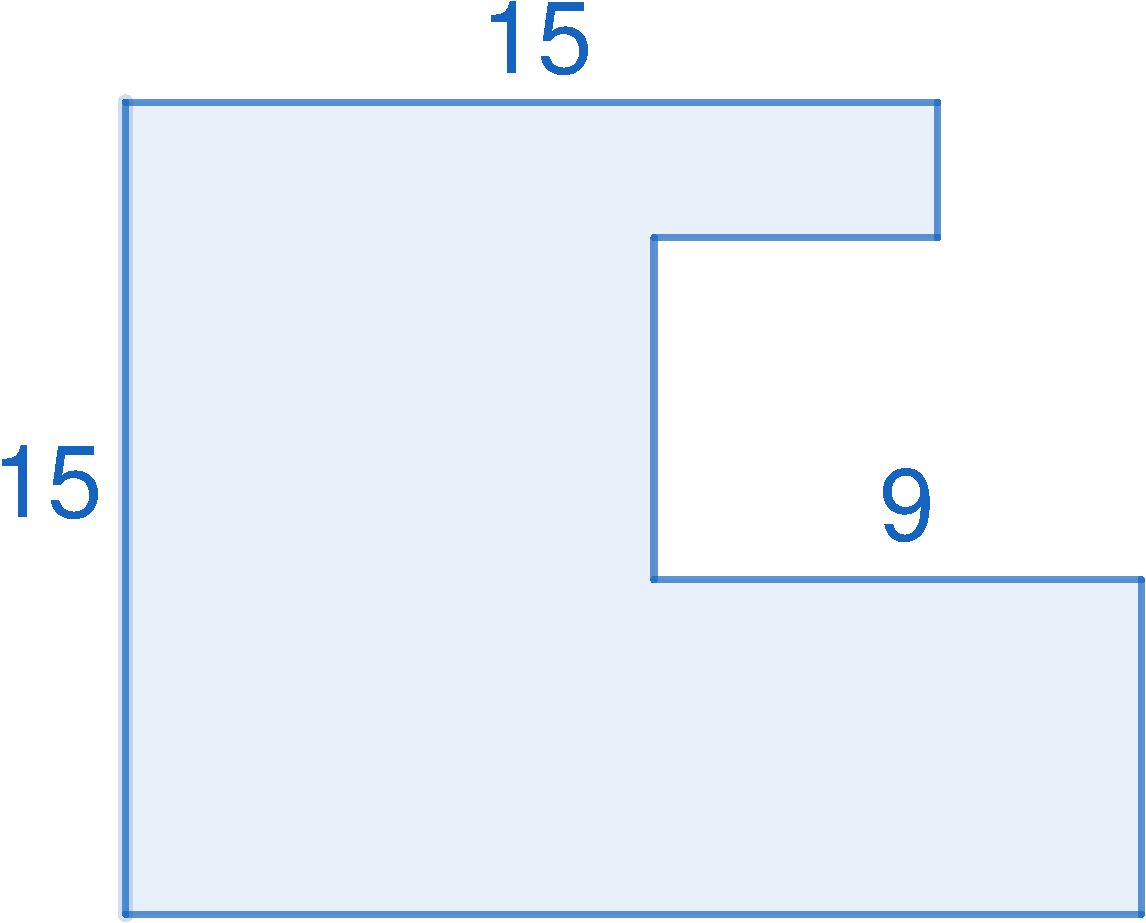
\includegraphics[height=4.2cm]{images/FinalProject-fig02.pdf}\par
	\end{center}
	
	%%  10  %%
	\item $B$ fourths, $C$ halves, and 9 sixteenths are all equal. The sum of $B+C$ is \raisebox{-3pt}{\rule{0.5in}{1pt}}.
	
	%%  11  %%
	\item $2^{200}-2^{199}-2^{198}-2^{197}-2^{196}$ equals what power of 2?
	
	%%  12  %%
	\item In the subtraction problem below, each time a letter appears it represents the same digit. Different letters represent different digits. Find the 4 digits representing TIME. HINT: both E and T are greater than 5.
	\begin{center}
		\begin{tabular}{cccccc}
				& E & M & I & T & \tabularnewline
			$-$ & M & I & T & E & \tabularnewline
			\hline 
				& T & I & M & E & \tabularnewline
		\end{tabular}\par
	\end{center}
	
	%%  13  %%
	\item What is the remainder when $3^{124}$ is divided by 5?
	
	%%  14  %%
	\item Mari has $B$ birds in her yard. If $K$ more birds were to land in her yard, there would be 3 times as many birds as there are now. In terms of $K$, how many birds are in Mari's yard?
	
	%%  15  %%
	\item $\langle a,b,c\rangle$ means ${\displaystyle \frac{b-c}{a-b}}$. For example, ${\displaystyle \langle8,6,10\rangle=\frac{6-10}{8-6}=\frac{-4}{2}=-2}$. Find all pairs $(x,y)$ so that $\langle x,9,y\rangle=4$ where $x$ and $y$ are whole numbers.
	
	%%  16  %%
	\item What is the units digit of $8^{88}$?
	
	%%  17  %%
	\item If $a\diamondsuit b=(a+b)-(b-a)$ and $a@b=7\left[(a+b)^{2}\div(a-b)^{3}\right]$, express $8\diamondsuit(10@12)$ in simplest form.
	
	%%  18  %%
	\item How many ways are there to make two 3-digit numbers whose sum is 670 using 6 different digits from 1 to 7? What are they? Is there a digit that isn't used in any of the addends?
	
	%%  19  %%
	\item A trapezoid and a rectangle have the same height. The larger base of the trapezoid is twice the length of the shorter base and equal to the length of the base of the rectangle. The base of the rectangle needs to be reduced by what percentage so that the two shapes have the same area?
	\begin{center}
		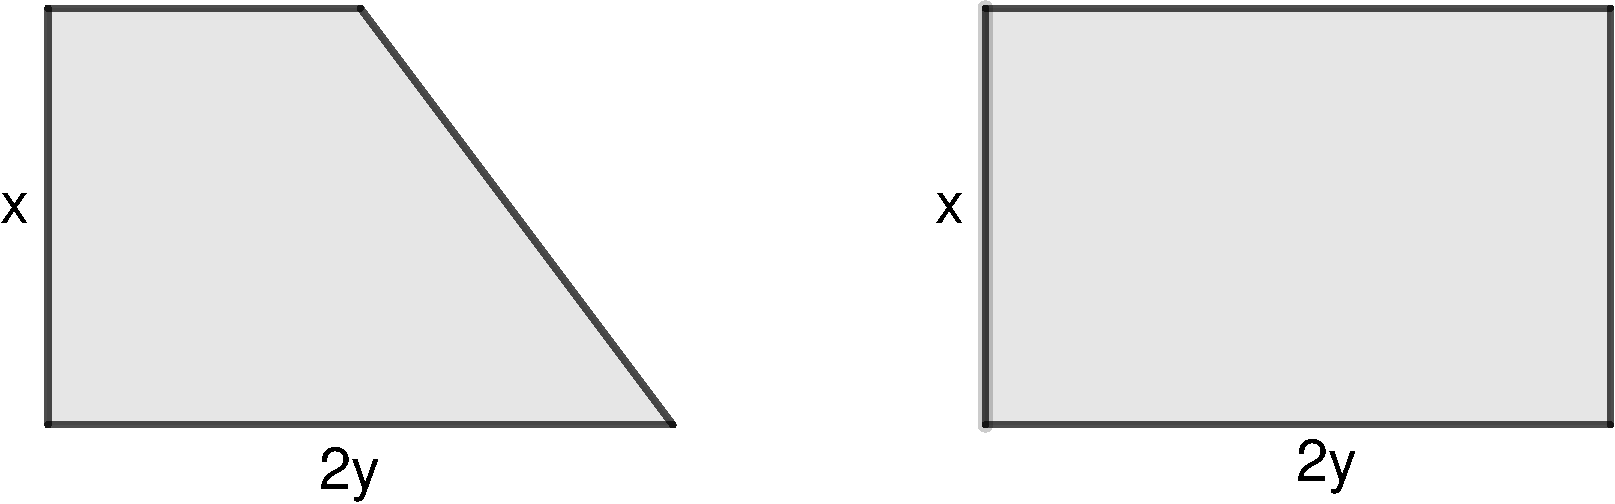
\includegraphics[height=4.2cm]{images/FinalProject-fig01.pdf}\par
	\end{center}
	
	%%  20  %%
	\item There are 12 people in a chess league that meets once per week. During the six-week season, each person will play at most one game in any week and will never play the same opponent twice.
	\begin{enumerate}
		\item If each player plays three games over the course of the season, how many games of chess will be played? Create a schedule for such a season.
		\item If each player plays six games over the course of the season, how many games of chess will be played? Create a schedule for such a season.
	\end{enumerate}
\end{enumerate}

\newpage
\Instr{ Solutions to these questions/hints you may provide students:
	\begin{enumerate}
		\item (sum of squares) Students are likely to simply try guessing and checking without a lot of success. There are simply too many possibilities. Considering that no sum will contain $17^2=289$ or any greater square, there are $_{16}C_{4}=1820$ possible combinations to choose from, making the chance of randomly guessing one about 0.7\%. The hint is supposed to encourage them to think in smaller chunks. Looking for sums that have a prescribed largest square boils the problem down to finding three perfect squares that sum to $270$ less that perfect square (and using only squares less than the prescribed one). For example, it makes quick work of finding all the combinations where the greatest square is $16^2=256$ since $270-256=14$ and it is easy to determine that there is exactly one way to write 14 as a sum of three squares ($1^2+2^2+3^2$). One can also use this idea to note that the largest square must be at least $10^2$ since $9^2+8^2+7^2+6^2=230<270$. Hence the largest square must be between $10^2$ and $16^2$. Seven searches for the remaining three squares is a much more tractable problem. The complete list is
		\begin{align*}
			5^{2}+8^{2}+9^{2}+10^{2} & =270\\
			2^{2}+8^{2}+9^{2}+11^{2} & =270\\
			6^{2}+7^{2}+8^{2}+11^{2} & =270\\
			1^{2}+1^{2}+11^{2}+12^{2} & =270\\
			1^{2}+5^{2}+10^{2}+12^{2} & =270\\
			3^{2}+6^{2}+9^{2}+12^{2} & =270\\
			1^{2}+6^{2}+8^{2}+13^{2} & =270\\
			2^{2}+4^{2}+9^{2}+13^{2} & =270\\
			4^{2}+6^{2}+7^{2}+13^{2} & =270\\
			1^{2}+3^{2}+8^{2}+14^{2} & =270\\
			3^{2}+4^{2}+7^{2}+14^{2} & =270\\
			2^{2}+4^{2}+5^{2}+15^{2} & =270\\
			1^{2}+2^{2}+3^{2}+16^{2} & =270\\
		\end{align*}
		It is not expected that students will find them all.
		
		\item (Mathemagician) Setting $x$ to be "the number, any number" chosen by an audience member, the operations prescribed can be summarized as
		$$\textrm{operate}\left[4(x+6)-x\right]-x=8$$
		Simplifying and rearranging this equation leaves
		$$\textrm{operate}\left[3x+24\right]=x+8$$
		so the missing operation must be "divide by 3". Students will more than likely not come to this conclusion this way, however. They are much more likely to simply try a few numbers and notice by the time they get to the unknown operation, they will need to divide by 3 and subtract the original number. Only a systematic record of starting number and trail through the operations will have a chance of revealing the answer.
		
		\item (Mr. Holiday) Mrs. Ehrlich was born in 1980. The only perfect square between 2000 and 2099 is $2025=45^2$, so she was/will be 45 in 2025. Mrs. Ehrlich's grandson was/will be born in 2046. The only other integer with an integer root between 2000 and 2099 is $2048=2^{11}$. This conclusion can be drawn by computing cubes, $4^{th}$ powers, $5^{th}$ powers, and so on, finding that
		\begin{itemize}
			\item $12^3=1728<2000<2099<2197=13^3$
			\item $6^4=1296<2000<2099<2401=7^4$
			\item $4^5=1024<2000<2099<3125=5^5$
			\item $3^6=729<2000<2099<4096=4^6$
			\item $2^7=128<2000<2099<2187=3^7$
			\item $2^8=256<2000<2099<3^7<3^8$
			\item $2^9=512<2000<2099<3^7<3^9$
			\item $2^{10}=1024<2000<2099<3^7<3^{10}$
			\item $2000<2^{11}=2048<2099$
		\end{itemize}
		
		\item (Mrs. Silver) By adding the cost for 5 lb nuts and 3 lb fruit to the cost for 3 lb nuts and 5 lb fruit, Mrs. Silver has the price for 8 lb of each. She simply divides this total in half to arrive at the price for 4 lb of each. Students will likely have to give themselves some numbers to work with before they catch on to this pattern.
		
		\item (The Klebes) The youngest Klebe will be 6 when the oldest is thrice their age (18). This can be derived by simple algebraic or non-algebraic methods by noting that the difference in their ages is 12. Whether the equation $3x=x+12$ (where $x$ is the age of the youngest) is used or not, students can generally land on this answer without too much trouble. Braden and Jaden are a different matter. With lots of poking around and trying different age differences, students may realize the fact that when Jaden's age is a factor of the difference between their ages, the quotient (Braden's age)/(Jaden's age) is an integer. It is exactly $$\frac{\textrm{age difference}}{\textrm{factor}}+1$$ Thus for there to be times when the older is twice, three times, and five times as old as the younger, the difference in their ages must be divisible by 1, 2, and 4, and therefore must be a multiple of 4. So the possible age differences are 4, 8, 12, 16, 20, 24, and so on up to some reasonable difference. It isn't likely that siblings will differ in age by more than 20 years, though this is a matter for debate. As long as students take the practical matter that siblings share parents and those parents are only fertile for a finite amount of time into consideration, it should be fine.
		
		\item (Numeration) The weird and different numeration system is base 3 where $\heartsuit=2,\ \triangle=1,\ \bot=0$, though the term "base 3" is intentionally absent because it has a tendency to lead students to looking up numeration in other bases, turning it into a research project instead of a problem solving project.
		$$\triangle\heartsuit\heartsuit\bot-\triangle\triangle\bot\bot=1220_3-1100_3=51_{10}-36_{10}=15_{10}$$ which can also be arrived at by doing the subtraction in base 3 first and then converting:
		$$\triangle\heartsuit\heartsuit\bot-\triangle\triangle\bot\bot=\triangle\triangle\bot=15_{10}$$
		Students simply need to observe and catch on to the pattern developed in the examples.
		
		\item ($x>1$) The equation $x-y=xy$ can be solved for $x$ or $y$, but the most immediate route to an answer is to solve for $y$:
		$$y=\frac{x}{x+1}$$
		Since $x>1$, $\frac12\leq y<1<x$. Consequently, the only correct answer is (b) $y<x$. The implication in the statement of this problem is that the answer does not depend on particular values of $x$ and $y$, so a student may simply choose a value of $x>1$ and solve for $y$ to determine the answer. However, this should also be accompanied by some explanation as to why the particular values do not matter (perhaps a whole bunch of examples?).

		\item (Aquarium) Setting $A$ as the price of an adult ticket and $C$ the price of a child ticket, we have $4A+5C=160$, and solving for $A$, 
		$$A=40-\frac54 C$$
		Because both ticket prices are in whole dollars, $C$ must be a multiple of 4, making the possible ticket prices
		\begin{center}
			\begin{tabular}{|c|c|c|c|c|}
				\hline
				$C$	& 4 & 8 & 12 & 16 \\
				\hline
				$A$ & 35 & 30 & 25 & 20 \\
				\hline
				discount & $\approx 88.57\%$ & $\approx 73.33\%$ & $52\%$ & $20\%$\\
				\hline
			\end{tabular}\par
		\end{center}
		Higher prices for the child ticket are not possible since they would require the adult ticket to be cheaper. If the percentage discount must be a multiple of 10, then the price of the child ticket is \$16 as can be seen from the chart. Students will hopefully find their way to these answers through exploration, organization, and analysis. They are not likely to do it algebraically as above.

		\item (Factorial) The word factorial is avoided intentionally. $1443=37\cdot 39$ so
		\begin{align*}
			\frac{1}{1443}\cdot\frac{40!}{\left(35!\right)\left(5!\right)} & =\frac{40\cdot39\cdot38\cdot37\cdot36\cdot35\cdot34\cdots2\cdot1}{39\cdot37\left(35\cdot34\cdot33\cdots2\cdot1\right)\left(5\cdot4\cdot3\cdot2\right)}\\
			& =\frac{40\cdot38\cdot36}{5\cdot4\cdot3\cdot2}=38\cdot12=456
		\end{align*}
		Students should write out the factorials and see all the cancelation. This is a great place to practice "solve a simpler problem first". If they simply decrease the numbers 40 and 35 to something manageable like 8 and 5 they might catch on to a pattern.
		
		\item (Perimeter) The lengths of the unlabeled vertical sides, shown in green below, cannot be determined individually, but altogether their length is clearly 15 units (same total length as the lefthand side of the octagon). Similarly with the horizontal sides shown in black. Their lengths cannot be determined individually, but together their length is clearly 9, leaving the left part of the bottom side at 15 units. These observations make it easy enough to calculate the perimeter:
		$$4\cdot15+2\cdot9=78$$
		\begin{center}
			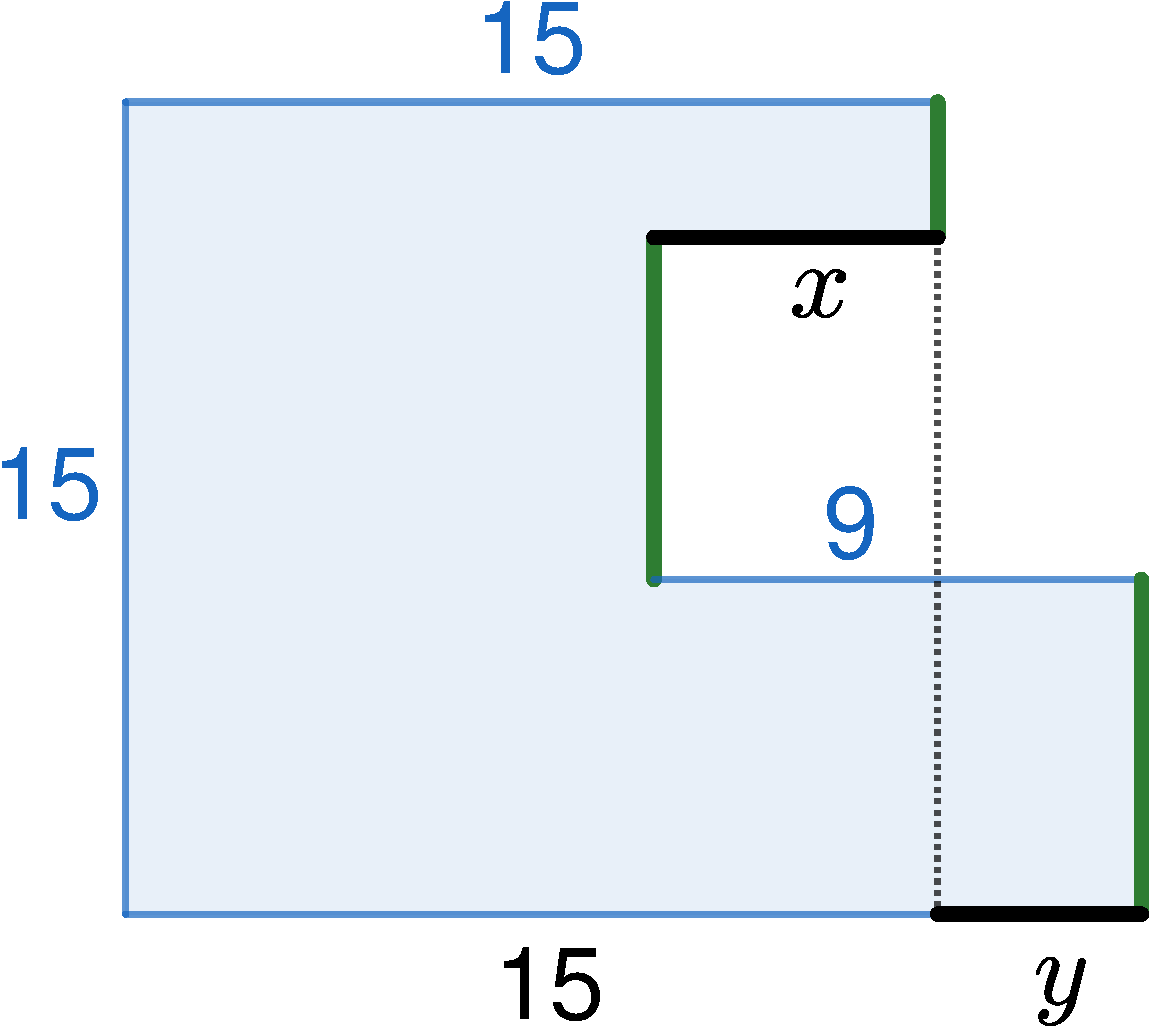
\includegraphics[height=5cm]{images/FinalProject-fig02-solution.pdf}\par
		\end{center}
		
		\item (9 sixteenths) Simply put, ${\displaystyle\frac{B}{4}=\frac{C}{2}=\frac{9}{16}}$, so ${\displaystyle B=\frac94}$ and ${\displaystyle C=\frac98}$. Therefore
		$$B+C=\frac94+\frac98=\frac{27}{8}$$
		This problem has a habit of confusing students since they expect $B$ and $C$ to be integers as they are numerators of fractions. It takes some facility with arithmetic to work with these compound fractions.
	
		\item (Powers of 2) The answer is 196 and can be derived in one of at least two different ways.
		\begin{enumerate}
			\item $2^{200}-2^{199}-2^{198}-2^{197}-2^{196}=2^{196}(2^4-2^3-2^2-2-1)=2^{196}$
			\item With some investigation, students can make the observation that the difference between consecutive powers of two is simply equal to the lesser power of 2 ($32-16=16$, $8-4=4$, and so on). Hence $2^{200}-2^{199}=2^{199}$ and $2^{199}-2^{198}=2^{198}$, and so on until the difference is determined to be $2^{196}$.
		\end{enumerate}
		This second solution can be arrived at by solving a simpler problem first!
		
		\item (TIME) Students must understand that the difference shown is a subtraction involving three 4-digit numbers, so borrowing is allowed (and necessary). Also, the digit 0 can (and must) be used. These are things that may not be immediately obvious to them. At least two observations can help narrow down the possibilities:
		\begin{itemize}
			\item Because $E$ is greater than 5, $E+E>10$, and the ones column, where we see $E+E=T$ (sort of) must require borrowing. The only numbers $E$, when doubled, that give a ones digit greater than 5 are $E=8$ and $E=9$, so we have either (a) $E=8;\ T=6$ or (b) $E=9;\ T=8$.
			\item The thousands digit suggest that either $T+M=E$ or $T+M=E-1$, depending on whether one has been borrowed from the $E$. In other words, $M=E-T$ or $M=E-T-1$. Combining this with the above observation, $M=0,1,\textrm{ or } 2$. Being a leading digit would suggest $M$ is either 1 or 2.
		\end{itemize}
		There are no more than 4 possibilities that follow from here, and they can be tested by trial and error. The one that works is
		\begin{center}
			\begin{tabular}{cccccc}
					& 9 & 1 & 0 & 8 & \tabularnewline
				$-$ & 1 & 0 & 8 & 9 & \tabularnewline
				\hline 
					& 8 & 0 & 1 & 9 & \tabularnewline
			\end{tabular}\par
		\end{center}
		
		\item ($3^{124}\div 5$) The answer is 1. Students who solve this using modular arithmetic almost certainly got help with this question. The most immediate path to a solution is to crank out the first bunch of powers of 3 and divide them by 5, noting the remainder:
		\begin{center}
			\begin{tabular}{|c|c|c|c|c|c|c|c|c|c|}
				\hline
				$n$				& 1 & 2 & 3 & 4 & 5 & 6 & 7 & 8 & 9 \tabularnewline
				\hline
				$3^n \mod 5$ 	& 3 & 4 & 2 & 1 & 3 & 4 & 2 & 1 & 3\tabularnewline
				\hline
			\end{tabular}\par
		\end{center}
		With a repeating cycle of 4, it is apparent that when the exponent is a multiple of 4, as is $124$, the remainder is 1. This question should not be given to anyone who is doing the question on the units digit of $8^{88}$.
		
		\item The answer is $K/2$. In the hypothetical situation that $K$ birds land, it triples the total, meaning twice as many birds landed as were already there. This conclusion can be reached by algebra, $B+K=3B\Rightarrow B=K/2$, or by drawing a diagram with the original birds set in black and the newcomers set in some other color. The diagram should make it apparent that the original number of birds is half the number of newcomers.
		
		\item ($\langle a,b,c\rangle$) Using some algebra,
		$$\langle x,9,y\rangle = \frac{9-y}{x-9}=4$$
		so $4x+y=45$. Since $x$ and $y$ are whole numbers, there is a finite collection of solutions:
		\begin{center}
			\begin{tabular}{|c|c|c|c|c|c|c|c|c|c|c|c|}
				\hline
				$x$		&  1 &  2 &  3 &  4 &  5 &  6 &  7 &  8 & 9 & 10 & 11 \tabularnewline
				\hline
				$y$ 	& 41 & 37 & 33 & 29 & 25 & 21 & 17 & 13 & 9 &  4 & 1  \tabularnewline
				\hline
			\end{tabular}\par
		\end{center}
		A couple of these solutions can be found by guess-and-check, but eventually the student should see a pattern and use that to make the complete list.
		
		\item ($8^{88}$) The answer is 6. Students who solve this using modular arithmetic almost certainly got help with this question. The most immediate path to a solution is to crank out the first bunch of powers of 8 and observe their units digits:
		\begin{center}
			\begin{tabular}{|c|c|c|c|c|c|c|c|c|c|}
				\hline
				$n$				& 1 & 2 & 3 & 4 & 5 & 6 & 7 & 8 & 9 \tabularnewline
				\hline
				$3^n \mod 5$ 	& 8 & 4 & 2 & 6 & 8 & 4 & 2 & 6 & 8\tabularnewline
				\hline
			\end{tabular}\par
		\end{center}
		With a repeating cycle of 4, it is apparent that when the exponent is a multiple of 4, as is $88$, the units digit is 6. This question should not be given to anyone who is doing the question on the remainder of $3^{124}\div 5$.
		
		\item ($8\diamondsuit(10@12)$) Students can muscle their way through this one by first calculating
		$$10@12=7[(10+12)^2\div (10-12)^3]=7\cdot\frac{22^2}{-2^3}=-\frac{847}{2}$$
		and then
		$$8\diamondsuit -\frac{847}{2}=\left(8+ \left(-\frac{847}{2}\right)\right)-\left(\left(-\frac{847}{2}\right)-8\right)=\cdots=16.$$
		However, this is likely to produce errors. Better that they realize, through observation or practicing with other numbers, that
		$$a\diamondsuit b=(a+b)-(b-a)=a+b-b+a=2a$$
		so $8\diamondsuit\ \textrm{anything}=16.$
		
		\item (Sum of 670) Three observations make the search fairly quick. (i) the ones digits must sum to 10, so are either (3 and 7) or (4 and 6); (ii) The tens digits must sum to 6 (because the one that carries from the ones digits will then give 7), so are either (1 and 5) or (2 and 4); (iii) The hundreds digits must also sum to 6, so they will be made from whichever pair is not used for the tens digits. A tree diagram is helpful in keeping all this straight and leads to the 6 sums
		$$\begin{gathered}
			143+527\qquad123+527\qquad127+543\\
			147+523\qquad217+453\qquad257+413
		\end{gathered}$$
		
		\item (Trapezoid) Algebraically, note that the areas are $A_{trap}=\frac32xy$ and $A_{rect}=2xy$ so the trapezoid has area equal to
		$$\frac{\frac32xy}{2xy}=\frac34$$
		of the area of the rectangle. Hence the area of the rectangle needs to be reduced by $\frac14$ or 25\%. Reducing the base of the rectangle by 25\% accomplishes this.\par
		Geometrically, it is clear to see that the trapezoid covers $3/4$ of the rectangle, bringing us to the same conclusion.
		\begin{center}
			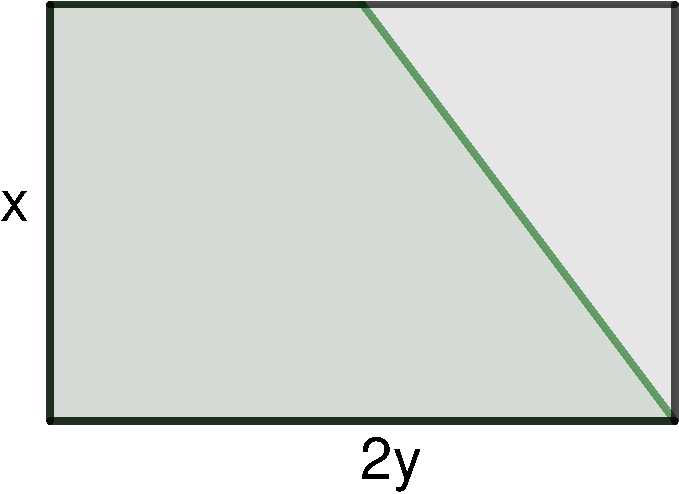
\includegraphics[height=5cm]{images/FinalProject-fig01-solution.pdf}\par
		\end{center}
		
		\item (Chess league) The number of games to be played is simple, though students will likely make it complicated. Double counting the games, we have that each person playing $n$ games requires $12n$ games. Since each game pits two players, the total number of games is half that, or $6n$. In a league where each player plays 3 games, that means $18$ games must be played, and where each player plays 6 games, $36$ games must be played. As for a schedule, a 3-game-per-person season is easiest to conceive by separating the 12 people into three groups of four. Each group plays a round robin tournament within their group (playing each person within the group once). Calling the people A-F, one possible schedule is
		\begin{center}
			\begin{tabular}{|c|c|c|c|c|c|}
				\hline
				wk 1 & wk 2 & wk 3 & wk 4 & wk 5 & wk 6\\
				\hline
				AB & GH & AC & FH & AD & FG\\
				\hline
				CD & IJ & BD & IK & BC & IL\\
				\hline
				EF & KL & EG & JL & EH & JK\\
				\hline
			\end{tabular}
		\end{center}
		This particular schedule has half the league playing each night with each player playing every other week. To create a schedule where each player plays six times is more difficult because it can not be done in a round robin fashion. However, the first three weeks can be made of the round robin inspired 3-game schedule by combining the first two weeks into one week, the 3rd and 4th weeks into another, and the 5th and 6th weeks into the third. Since no player has played any team from another group, new groups can be formed by mixing two players from one group with two players from another. Since each player will see two new people within their new group, two more games can be scheduled per person. Finally, the last week can be put together in any way that avoids a repeat matchup. One such schedule is
		\begin{center}
			\begin{tabular}{|c|c|c|c|c|c|}
				\hline
				wk 1 & wk 2 & wk 3 & wk 4 & wk 5 & wk 6\\
				\hline
				AB & AC & AD & AE & AF & AG\\
				\hline
				CD & BD & BC & BF & BE & BH\\
				\hline
				EF & EG & EH & CI & CJ & CK\\
				\hline
				GH & FH & FG & DJ & DI & DL\\
				\hline
				IJ & IK & IL & GK & GL & EI\\
				\hline
				KL & JL & JK & HL & HK & FJ\\
				\hline
			\end{tabular}
		\end{center}
	\end{enumerate}
}
